\chapter{Implementation and training}
\label{kap:implementation}

Because of its excellent machine learning support, we chose to write all of our code in Python and train all the models using the PyTorch framework \cite{pytorch} because of its straightforward setup for distributing training on multiple GPUs.
\newline
We've performed training on two powerful servers, both of them equipped with two NVIDIA GeForce RTX 2080 Ti graphic cards. Thanks to this graphic card's big RAM, we were able to fit reasonably large batch sizes, which significantly reduced training time and stabilized training across all models.
\newline
As PyTorch does not support any visualization of the training process out of the box, we integrated Tensorboard into our training procedure, logging training and validation error after each epoch of training, of which an example is shown in figure \ref{fig:tesorboard}.
\begin{figure}[H]
    \centerline{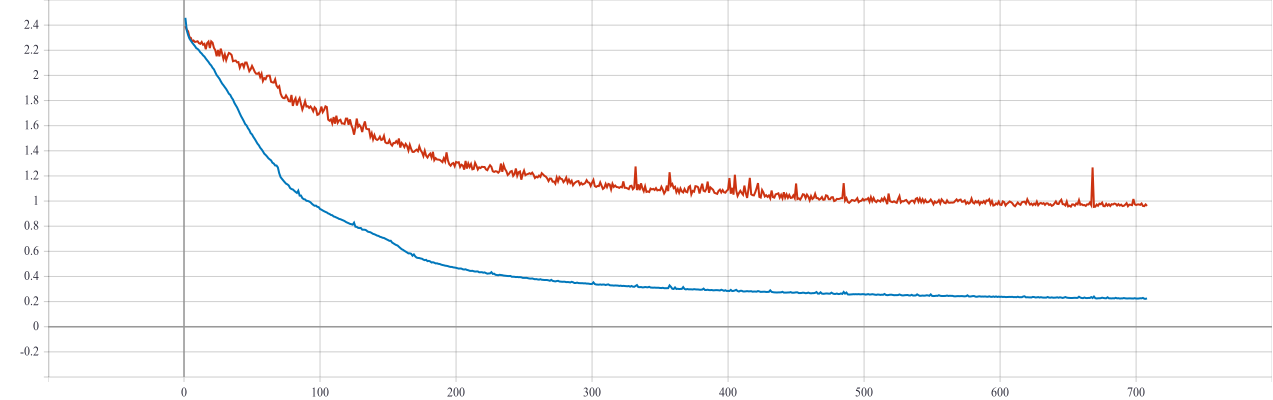
\includegraphics[width=0.6\textwidth]{praca/images/Training-IRN.png}}
    \caption[Our Tensorboard logging setup]{Our Tensorboard logging setup, with training (blue) and validation (red) error}
    \label{fig:tesorboard}
\end{figure}
\section{Training procedure}
Following training procedure suggested in \cite{sengupta-inverse-rendering}, we started training EnvMap net, first on images synthesized by direct renderer presented by Sengupta et al. and then fine-tune it on raytraced images with loss functions specified in the original paper. With trained EnvMap net, we generated ground-truth environment map for each image in our dataset. As we have explained in chapter \ref{kap:approach}, using their direct renderer did not work well on our data, as our images were rendered not only with diffuse but also specular materials, which caused problems. We realized this problem after we trained and fine-tuned the model, so we had to retrain it from scratch.
\newline
With all the ground-truth data ready, we trained IRN with the following loss: 
\begin{equation}
\begin{split}
    L_{IRN} = \|\hat{N} - N^* \|_1 + \|\hat{D} - D^* \|_1 + \|\hat{G} - G^* \|_1 + \|\hat{V} - V^*\|_1 + \|\hat{S} - S^*\|_1 \\ 
    + \; \frac{\|f_{Phong}(D^*, N^*, \hat{L}, G^*, V^*, S^*) - f_{Phong}(D^*, N^*, L^*, G^*, V^*, S^*)\|_1}{2}
\end{split}
\end{equation}
where $^*$ stands for ground-truth data, $\hat{}$ stands for predicted data, $N, D, G, V, S$ correspond to surface normals, diffuse albedo, glossiness, view vector and specular albedo respectively and $f_{Phong}$ denotes our Phong direct render function, as specified in chapter \ref{kap:approach}.
\newline
To train RAR
\begin{equation}
    I_r = RAR(I)
\end{equation}
we adjusted the original RAR loss to account for our new direct renderer as
\begin{equation}
    L_{RAR} = \| I - (I_r + f_{Phong}(\hat{D}, \hat{N}, \hat{L}, \hat{G}, \hat{V}, \hat{S})) \|
\end{equation}
where $I$ denotes input image and $\hat{D}, \hat{N}, \hat{L}, \hat{G}, \hat{V}, \hat{S}$ image properties estimated by IRN.
\newline
We chose Adam \cite{adam} as our optimizer for minimizing cost function, as this optimization method outperformed all other methods by constantly giving lower training and validation error. All models were optimized with learning rate $\alpha = 0.001$.
\newline
The time required to fully train the model varied between architectures, from 2 days for the smaller ones to one week for IRN.